
%%%%%%%%%%%%%%%%%%%%%%% file typeinst.tex %%%%%%%%%%%%%%%%%%%%%%%%%
%
% This is the LaTeX source for the instructions to authors using
% the LaTeX document class 'llncs.cls' for contributions to
% the Lecture Notes in Computer Sciences series.
% http://www.springer.com/lncs       Springer Heidelberg 2006/05/04
%
% It may be used as a template for your own input - copy it
% to a new file with a new name and use it as the basis
% for your article.
%
% NB: the document class 'llncs' has its own and detailed documentation, see
% ftp://ftp.springer.de/data/pubftp/pub/tex/latex/llncs/latex2e/llncsdoc.pdf
%
%%%%%%%%%%%%%%%%%%%%%%%%%%%%%%%%%%%%%%%%%%%%%%%%%%%%%%%%%%%%%%%%%%%


\documentclass[runningheads,a4paper]{llncs}

\usepackage{amssymb}
\setcounter{tocdepth}{3}
\usepackage{graphicx}
\usepackage{bm}
\usepackage{multirow}

%\usepackage{url}
%\urldef{\mailsa}\path|{alfred.hofmann, ursula.barth, ingrid.haas, frank.holzwarth,|
%\urldef{\mailsb}\path|anna.kramer, leonie.kunz, christine.reiss, nicole.sator,|
%\urldef{\mailsc}\path|erika.siebert-cole, peter.strasser, lncs}@springer.com|    

\newcommand{\keywords}[1]{\par\addvspace\baselineskip
\noindent\keywordname\enspace\ignorespaces#1}

\begin{document}

\mainmatter  % start of an individual contribution

% first the title is needed
\title{Demographic analysis of websites preferences on mobile devices by respondents involved through motivational activities}


% a short form should be given in case it is too long for the running head
\titlerunning{Demographic analysis of websites preferences}


%\thanks{Please note that the LNCS Editorial assumes that all authors have used
%the western naming convention, with given names preceding surnames. This determines
%the structure of the names in the running heads and the author index.}%

% the name(s) of the author(s) follow(s) next
\author{Iskander Kareev, Rustem Salimov, Darya Lavrova, Ruslan Gaisin}
%
\authorrunning{Iskander Kareev, Rustem Salimov, Darya Lavrova, Ruslan Gaisin}
% (feature abused for this document to repeat the title also on left hand pages)

% the affiliations are given next; don't give your e-mail address
% unless you accept that it will be published
\institute{Kazan Federal University}
%Springer-Verlag, Computer Science Editorial,\\
%Tiergartenstr. 17, 69121 Heidelberg, Germany\\
%\mailsa\\
%\mailsb\\
%\mailsc\\
%\url{http://kpfu.ru/eng}}

%
% NB: a more complex sample for affiliations and the mapping to the
% corresponding authors can be found in the file "llncs.dem"
% (search for the string "\mainmatter" where a contribution starts).
% "llncs.dem" accompanies the document class "llncs.cls".
%

\toctitle{toc title}
\tocauthor{toc author}
\maketitle

\begin{abstract}
The purpose of this research is demographic analysis of users who participated in motivational events and their web-site preferences. The information on web actitivity and social attributes of the users were accumulated by means of application "Sazan SRR". The study was conducted using such demographic characteristics as marital status, gender, age category and occupational status. The analysis consisted of the users set clusterization on the basis of the aforementioned attributes with control of the visited sites, and on the pair-wise independence testing. The study revealed some interesting statistical connections, namely, high influence of age of the responders on which of the sites they visit.


\keywords{data mining, clusterization, clusters interception measure, demographic analysis, independence tests}
\end{abstract}


\section{Introduction}

The problem of social and demographic statistical analysis of people behavior and preferences are of highest interest in many spheres, such as marketing, politics, city management and so on. In our study we conducted such analysis for the demographic and web-activity of users collected through special software on basis of motivational events on social nets. Some of the similiar demographic analysis studies are \cite{sim-1}, \cite{sim-2}.

The analysis consisted of two mutually complementary studies. The first one is a clusterization of the users based on their demographic attributes (marital status, gender, age category and occupational status) with control of the set of web-sites visited by people within each of the generated clusters. The second study consisted in a pair-wise dependency testing between each of the demographic attributes and the fact of visiting a web-site category.

The investigation revealed some interesting relationship between users attributes and their web-sites preferences. Namely, that the age of the users have the most statistical influence on their Internet sites preferences. 

The computational part of the study were done with usage of R software environment for statistical computing and graphics \cite{r-project}


\section{Used data collection and their description}\label{the-description}


\subsubsection{Data collection.}
Material reward, as is known, is one of the best people motivations to take part in some actions. So it was decided to motivate future research group by means of raffle prizes.
A lot of advertisements in 20 groups with large quantity of members about participation in large-scale scientific research which provides an opportunity to win great prizes were placed. Also activists of student labor teams lead intramural performances inside schools, universities and colleges, activists of student labor teams lead intramural performances.
\\* To carry out research successfully more than 600 of respondents were required. They send information during 10 weeks.
\subsubsection{Data description.}
As the input data there was a base of Internet-users with several characteristics obtained through the usage of application "Sazan SRR" by them.  The application analyzes a history of browser and use it to compute interest categories (as a list of categories Yandex categories are taken). To improve the process of work and analysis the application asks user to fill out a form and sends the information to the server. 
\\* Sazan analyzes following data to build user profile: Location (GPS coordinates, mobile network cell ID), History Web (URL (address) of visited Web-page, Web-page header, time of visiting), Usage application history (Application ID, Application launch time, Application launch duration), Wi-Fi (wireless network connection name, MAC-address hash code of the network), Bluetooth (connected device name, MAC-address hash code of the network), Battery (battery value, time connection/disconnection of battery charger), Screen (lock/unlock time).
\\* As a result of data structuring the table containing the following fields was received: uid - user ID, timestamp - time of visiting, date - date of visiting, visits - number of visits, title - Web-page header, url - address of visited Web-page.



\subsubsection{Data pre-processing.}\label{the-treatment}
Users with missing characteristics values were excluded before conducting research. Websites names were extracted from the initial URL of the user queries. URL which are not  Web-page addresses (appeal to local data, chrome-queries etc.) were removed. In this way, further research was reduced to only «normalized» URL sites.
\\* The original table was transformed into a selection containing the following fields: webapi agecateg - user's age, gender - gender, marital - marital status, jposition - occupational status.
\\* After pre-processing the selection comprises 316000 URL sites and 526 users. 
To improve the robustness of the investigation and clearness of its results a list of sites was initially filtered so that only sites with not less 5 visits were remained.



\section{Clusterisation of users by demographic attributes}

The goal was to provide the clusterisation of the set of users on several groups based on their demographic attributes (like age, occupational status and so on) and the sites they visited. The expectation was to get an interpretable insight on the connection between users' social status and their preferences on Internet sites. 





\subsubsection{Notion and attributes recoding.}

Let $U$ be the set of all users in the dataset and $S$ be the set of all sites (urls). By $S(u)$ denote the set of all sites which were visited by user $u \in U$. By $S(A)$ denote the set of all sites which were visited by at least one user from the set $A \subset U$. By $U(s)$ denote the set of all users which visited site $s \in S$.


The investigation was done using the following demographic attributes: marital status ($a_1$), gender ($a_2$), age category (denoted as $a_3$) and occupational status ($a_4$). So to each $u \in U$ a vector of attributes $\boldsymbol{a} = (a_1, a_2, a_3, a_4)$ is assigned.

For simplicity of application of common clusterisation algorithms and to preserve the natural order of the values, all of the demographic attributes were recoded from categorical to numerical format in the following way:


\begin{itemize}
\item for $a_1$ (\textit{marital} column in original dataset): \\ 
	``\textit{Single}''  $\to$ 0,  \qquad  ``\textit{In relations}''  $\to$ 0.5, \qquad  ``\textit{Married}''  $\to$ 1;
	\smallskip
	
\item for $a_2$ (\textit{gender} column in original dataset): \\ 
	``\textit{Male}''  $\to$ 0, \qquad  ``\textit{Female}'' $\to$ 1;
	\smallskip
	
\item for $a_3$ (\textit{webapi\_agecateg} column in original dataset): \\ 
	``\textit{0..17}''  $\to$ 1, \qquad  ``\textit{18..24}''  $\to$ 2, \qquad     ``\textit{25..34}''  $\to$ 3, \qquad  ``\textit{35..44}''  $\to$ 4, \\     ``\textit{45+}''  $\to$ 5;
	\smallskip
		
\item for $a_4$ (\textit{jposition} column in original dataset): \\ 
	``\textit{employee}'' $\to$ 1, \qquad  ``\textit{executive}'' $\to$ 1, \qquad  ``\textit{jobless}'' $\to$ 0, \\  ``\textit{minor}'' $\to$ 0, \qquad  ``\textit{student}'' $\to$ 0.5.
\end{itemize}

The clusterisation of $U$ is done by the values of attributes $(a_1, a_2, a_3, a_4)$ using complete linkage hierarchical clustering \cite{hclust} with Euclidean distance. Let us note that the clusterisation were done using \textit{hclust} method of \textit{R} statistical package. Since those algorithm are sensitive to the scale of the data, the attributes $a_1$, $a_2$, $a_3$, $a_4$ are rescaled to have zero mean and unit variance throughtout the dataset. We denote the values of the attributes after recoding and rescaling by $\boldsymbol{x} = (x_1, x_2, x_3, x_4)$.

Due to aforementioned sensitivity of the clusterisation algorithm to the scale of input variables, we can regulate the importance of each of the attributes by bringing in weights $\boldsymbol{w} = (w_1, w_2, w_3, w_4)$ where \quad $w_i \in [0, 1], \quad i = 1,2,3,4$. Thus the clusterisation is done on the values of vector $(w_1 x_1, w_2 x_2, w_3 x_3, w_4 x_4)$.

Let $k$ be the number of clusters on which $U$ supposed to be clusterised. By $\mathfrak{C}(\boldsymbol{w}, k)$ denote the resulting clusterisation for given $k$ and weights $\boldsymbol{w}$, so
\[
	\mathfrak{C}(\boldsymbol{w}, k) = \{C_1, C_2, \dots, C_k\} \  \colon  \quad  C_1 \cup C_2 \cup \dots \cup C_k = U.
\]

Let $S_i = S(C_i)$ --- the image of users clustarisation $\mathfrak{C}(\boldsymbol{w}, k)$ to the set of all sites $S$. We want to pick values of weights in such way that the sets $S_1, ..., S_k$ are well separated and there is no much intersection between them, i.e. our clusterisation results in users clusters which are well distinguishable in terms of the sites users visit. In the following our approach to that task is described.



\subsubsection{Weights and sites intersection measure.}

Suppose the number of clusters $k$ is fixed. Let us describe the algorithm for choosing weights $\boldsymbol{w}$. Let
\[
	r_{s,j} = \frac{\mathcal{N}(U(s) \cap C_j)}{\mathcal{N}(C_j)},
\]
where $s \in S$, $C_j \in \mathfrak{C}(\boldsymbol{w}, k) \quad (1 \leq j \leq k ),$ and $\mathcal{N}$ is the number of elements in its argument.

By means of $r_{s,j}$ we define an intersection measure for the clusterisation $\mathfrak{C}(\boldsymbol{w}, k)$:
\[
	M_I = \sum_{s \in S} \Big( \sum_{j=1}^{k} r_{s,j} - \min_{j\colon 1 \leq j \leq k} r_{s,j} \Big).
\]
Measure $M_I$ adds a ``penalty'' for sites which are visited by users from several different clusters.

We choose the weights $\boldsymbol{w}$ as the ones for which $M_I$ is minimised. We solve this minimisation problem computationally with the precision of 0.2 points.



\subsubsection{Clusters number $k$.}

In our investigation we studied the influence of clusters number $k$ to two parameters: the number of ``unique'' sites (i.e. the ones which occur only in one of the sets $S_j, \quad 1 \leq j \leq k$) and the value of the interception measure $M_I$ (for ``optimal'' weights $\boldsymbol{w}$). Those dependancies are depicted in Fig.~\ref{N7Jti}.

\begin{figure}

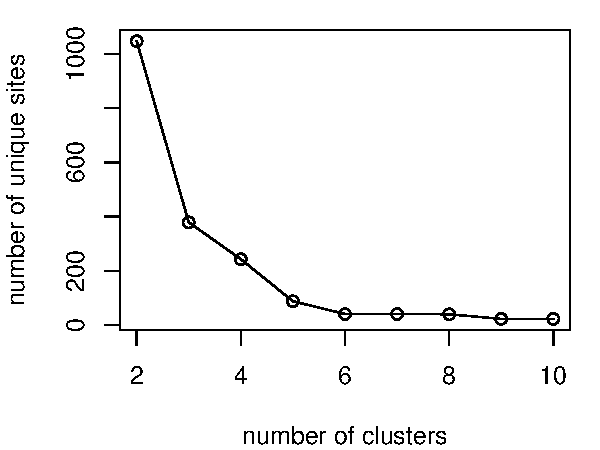
\includegraphics[scale=0.6]{fig_uurls.pdf}\hfill
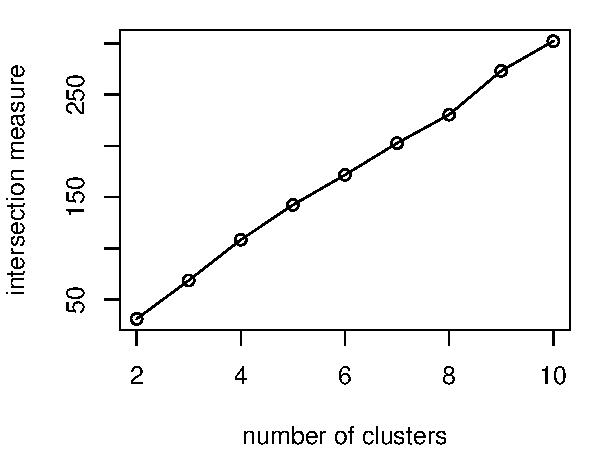
\includegraphics[scale=0.6]{fig_meas.pdf}

\caption{The number-of-unique-sites vs $k$ plot (on the left) and $M_I$ vs $k$ plot (on the right)}
\label{N7Jti}
\end{figure}

Taking into account the aforementioned parameters and after the AIC algorithm results (see \cite{aic}) we choose $k=6$ as the clusters number. For that $k$ the weights minimising the interception measure $M_I$ are found to be:
\[
	\boldsymbol{w} = (0.4, 0.4, 1.0, 0.4).
\]
Let us recall that the weight $w_3$ corresponds to the age of the user. Due to that we might suggest that the agehas the most the most distinguishing effect on the preference of the users for the Internet sites.


\subsubsection{The results and their interpretation.}

Some information on the resulting clusters are provided in Tables~\ref{OWoti} and~\ref{01Yti}. The Table~\ref{OWoti} contains the demographic composition of the clusters. The Table~\ref{01Yti} contains 10 subject categories of sites (the mapping of sites to the categories were done according to Yandex database) most specific to the relevant clusters.


\begin{table}
	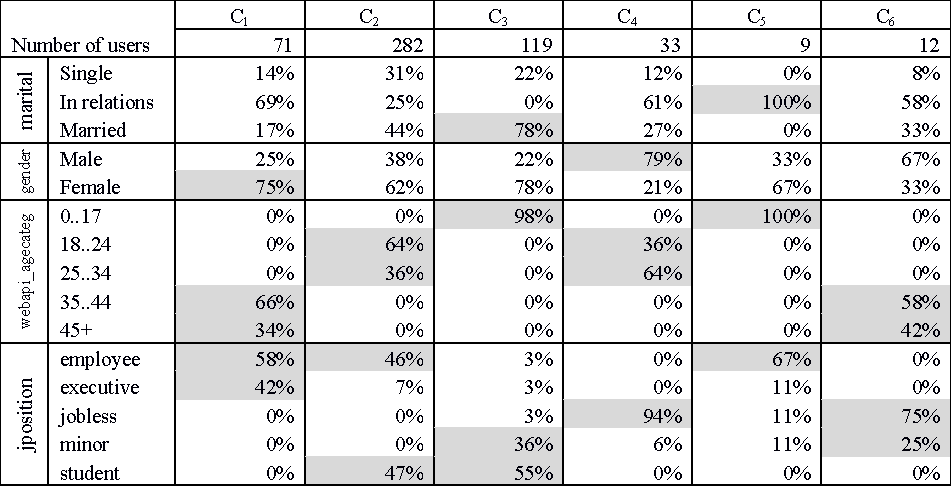
\includegraphics[width=\linewidth]{t1.pdf}
	
	\caption{The demographic composition of the clusters. The most distinctive attribute values for the clusters are greyed out.}
	\label{OWoti}
\end{table}





\begin{table}
	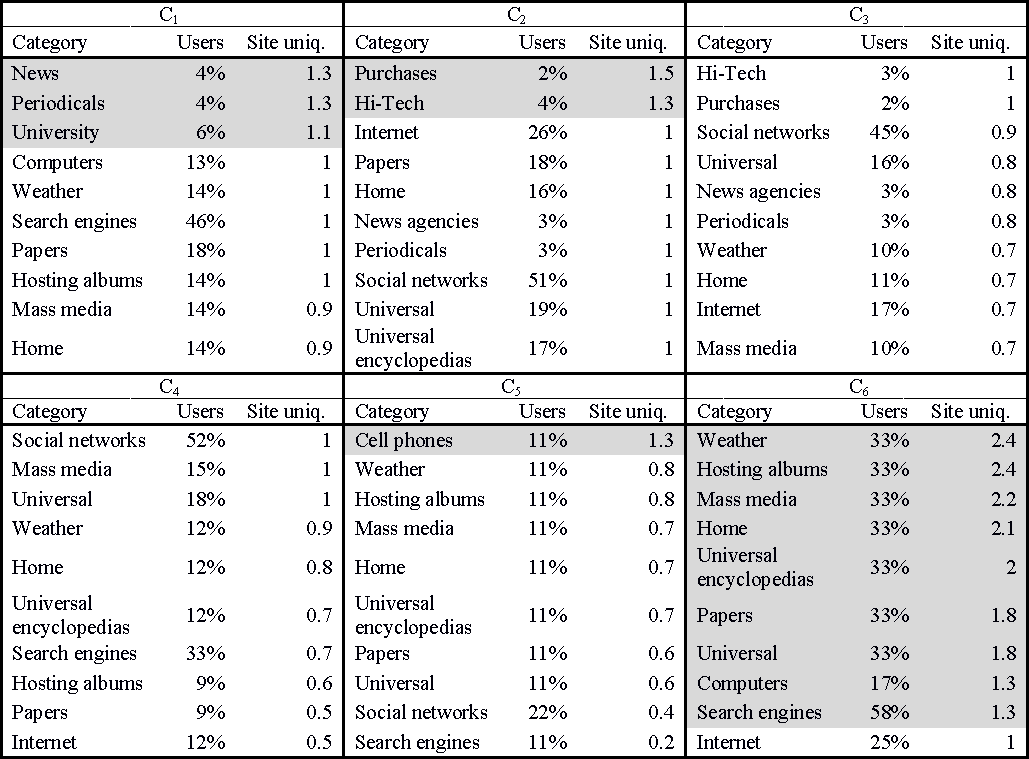
\includegraphics[width=\linewidth]{t2.pdf}
	
	\caption{Some of the categories of sites which are visited by the users of the relevant clusters. The column ``Users'' shows the proportion of users in the cluster which have visited the sites of the category. The column ``Site uniq.'' shows how mush the proportion of users for the category within this cluster is more than in any other cluster. }
	\label{01Yti}
\end{table}

Let us provide a brief description of some of the obtained clusters:
\begin{itemize}
	\item $C_1$ is mostly formed with aged working and unmarried women. It is distinctive for the class to visit news and periodicals sites, and be interested in universities.
    
    \item $C_2$ consists of young/middle-aged students and working people. Their distinctive sites are about Hi-tech and purchases.

	\item $C_5$ consists of working teenagers in relations with high interests on sites about mobile phones.
    
	\item $C_6$ is formed by aged jobless people with a lot of spare time, as it seems. Are wide variety of sites categories are highly distinctive to them, including weather, photo hosts, mass media, home and so on.
\end{itemize}

Let us note that the demographic data on the users were gathered by means of online interview without any test for correctness. The authenticity of the entered information remained on the conscience of respondents, so nobody can exactly say about reliability of obtained data. For instance, $C_3$ almost completely consists of married people who are under 17 years old which is unlikely to be true.


\section{Dependency analysis between demographic attributes of a users and sites they visited}



One of the problems was the task of checking the independence of the attributes of the data and sites categories. For this purpose chi-squared test is usually used if explored indications are qualitative. So we had to build a contingency tables and to make decisions about hypothesis of independence.

Originally it was planned to analyze the relationships between the features of respondents and visits to the sites. However, for most sites this version of the analysis is not suitable due to the fact that they have a small number of visits; the same time for the sites with big number of visits(vk.com, google.com, and so on) to allocate a significant relationship is not possible. Therefore, it was decided to group the original sites into categories for further analyzing. The categories with large number of visits (more than 1000) were selected for the analysis, because for the categories with fewer visits the study is not applicable due to the limitations of test. For each user and each category has been allocated fact of the visit (variable that possesses values 0 or 1). After that contingency tables were built and by these tables the hypotheses of independence were tested with a significance level 0.05.

It should be noted that two most popular categories: "Social networks", "Bots" - in which the number of visits by much more than in all other categories, depending on the features of the respondents users could not be found. That is a logical result, because websites of the most popular categories should be visited by users regardless of age, sex and other features. 

A little bit strange result is that a visit to any one of the categories doesn’t depend on the gender of the respondents. Perhaps this is due to a not enough large sample size.

Some interesting relations:

\begin{itemize}
	\item Between the \textbf{age} attribute and the category "\textbf{Newspapers}" (with a high significance level \textbf{0.0015}) The result shows the benefit of young people aged 0 to 24 years of age and older people 45+ are much more likely not visit sites category "Newspapers".
	\item Between the \textbf{marital status} and the category "\textbf{Dating}" (the significance level of \textbf{0.026}). As expected, unmarried single people visit sites "dating" category.
	\item Between the \textbf{age} attribute and category of websites "\textbf{Dating}" (with a high level of significance \textbf{0.009}). Older people visit dating sites are more likely than younger ones.
	\item Between the \textbf{age} attribute and the "Internet" category (with a high level of significance \textbf{0.01}). It confirms the assumption that young people are more likely to visit sites with such a category.
	\item Between the \textbf{age} attribute and category of "\textbf{Information Agency}" (with a significance level of \textbf{0.022}). Here we see an unclear relation: young people under the age of 17 years, significantly more likely to visit sites with the category News agencies.
	\item Between marital status and the category "\textbf{Shopping}" (a high level of importance of \textbf{0.0053}). Married people, or irrelevant, significantly more likely to visit sites category Shopping, in turn, single people opposite.
	\item Between the \textbf{age} attribute and the category of websites "\textbf{Work}" (the significance level of \textbf{0.013}). Young people were significantly more interested in work sites category.
	\item Between the \textbf{age} attribute and the category "\textbf{Universal Encyclopedia}" (high significance level \textbf{0.0023}). Young people between 18 and 24 years old visit sites og the category "Universal Encyclopedia" rare than younger participants (0..17) and slightly older participants (24..34).
	\item Between the \textbf{workplace} and the category "\textbf{Universal Encyclopedia}" (high significance level \textbf{0.0082}). For this feature the obvious relation that students use the sites of this category more often than other groups figured out again. Complete workers also use sites of this category.
	\item Between the \textbf{age} attribute and the category "\textbf{Humor}" (significance level \textbf{0.04}). For this category we get the obvious connection that young people aged 18 to 34 years visited sites category humor more often.
	\item Between the \textbf{labor} attribute and category of websites "\textbf{Humor}" (significance level \textbf{0.03}). The connection that students visit sites in this category more often is highlighted here.
\end{itemize}


\section{Conclusion}

In our study a statistical analysis were done for the demographic data bounded with some information on the web activity of the Internet users. Some original clusterization technique were considered. Its effectiveness was somewhat backed up by the fact that it revealed high influence of age of the responders on their web-sites preferences --- the same statement were obtained with chi-square independence test.


\subsubsection*{Acknowledgments.} This work was funded by the subsidy allocated to Kazan Federal University for the state assignment in the sphere of scientific activities.

\begin{thebibliography}{4}


\bibitem{aic} Akaike, H. (1973). "Information theory and an extension of the maximum likelihood principle", in Petrov, B.N.; Csáki, F., 2nd International Symposium on Information Theory, Tsahkadsor, Armenia, USSR, September 2-8, 1971, Budapest: Akadémiai Kiadó, pp. 267–281.


\bibitem{r-project} R Core Team (2016). R: A language and environment for statistical computing. R Foundation for Statistical Computing, Vienna, Austria. URL https://www.R-project.org/.


\bibitem{hclust} Rokach, Lior, and Oded Maimon (2005). "Clustering methods." Data mining and knowledge discovery handbook. Springer US.


\bibitem{sim-1} 
Sloan L., Morgan J., Burnap P., Williams M. Who Tweets? Deriving the Demographic Characteristics of Age, Occupation and Social Class from Twitter User Meta-Data. Preis T, ed. PLoS ONE. 2015;10(3):e0115545. doi:10.1371/journal.pone.0115545.


\bibitem{sim-2}
Stattner E., Collard M. (2017)
Clustering of links and clustering of nodes: Fusion of knowledge in social networks. Studies in Computational Intelligence, 665, pp. 255-276. 


\end{thebibliography}




\end{document}
